\chapter{Performance Evaluation of libtribler}
\label{chapter:experiments}

Technical debt has a negative impact on product quality in terms of defects and other structural quality issues\cite{tom2013exploration}: it is significantly harder to fix defects in a complex, unstructured system and more dangerous in a sense that one might introduce additional bugs when trying to fix one. Boosting performance is often achieved by minor or major refactoring efforts of system components to utilize another underlying model or structure. These kind of modifications are more involved when the system as whole is suffering from huge amounts of technical debt.\\\\
Now that we got rid of most technical debt identified in the Tribler core and user interface, the next step towards a stable, future-proof libtribler involves research efforts on the usability and performance of available components. We wish to quantify the performance of operations performed by users in libtribler to get an idea about the usability of the core in general. For various components such as the torrent lookup mechanisms we have no performance baseline to help us to make statements about usability. We will perform a number of experiments and for each experiment, we will present and discuss the observed results. We have two additional purposes with these experiments: on the one hand, we show that the performance of the system did not degrade to an unacceptable extent due to our refactoring efforts. On the other hand, we use the performance measurements to create a baseline and to identify possible failures or issues that we will document and classify as future work.

\section{Environment Specifications}
\label{sec:environment-specifications}
The experiments performed in this chapter are executed on a virtual private server (VPS). We wish to stay as close as possible to the specifications of a machine that an actual user could be using. A summary of the specifications of the configured machine used for most of the experiments described in this chapter, is given in Table \ref{table:experiments-server-specifications}.

\begin{table}[h!]
	\centering
	\begin{tabular}{|l|l|}
		\hline
		\emph{Processor} & Intel Xeon CPU E5-2450 (2.50GHz, 4 cores)\\ \hline
		\emph{Memory} & 8GB 1000MHz \\ \hline
		\emph{Storage} & 50GB \\ \hline
		\emph{Operating system} & Ubuntu 15.10 \\ \hline
	\end{tabular}
	\caption{The specifications of the machine used for most of the experiments.}
	\label{table:experiments-server-specifications}
\end{table}

\noindent The experiments are not executed in an isolated, artificial environment but are using the deployed Dispersy network. While the obtained results may be different between users, this set-up can be used to get more insights in the performance of Tribler from the perspective of the user.\\\\
If not stated otherwise, the default Tribler configuration file values are used. These default values are located in the \emph{defaults.py} file in the source code directory of Tribler\footnote{https://github.com/Tribler/tribler/blob/devel/Tribler/Core/defaults.py}. In the configuration file used during the experiments, all communities, except for the BarterCast community, are initialized. Dispersy, the REST API and the video server are enabled during the experiments. All experiments are executed without running the wxPython or Qt GUI.\\\\
Some of the experiments are built using a scenario file. In a scenario file each line specifies a specific command of a peer at a specific point in time during the experiment. Our framework used to run the experiments, Gumby, contains code to read scenario files, interprets the commands to be executed and to schedule these actions in Twisted. Several utility methods have been implemented to gather and write statistics to files in a processable and readable format that can be parsed by visualization tools such as R\footnote{https://www.r-project.org}. Various Dispersy experiments are already built using the scenario file framework, mainly in our \emph{AllChannel} experiment that runs on the DAS5 supercomputer. Before we execute the experiments in this chapter, we first extended the usability of the scenario files to run and manage a Tribler session and we improved the framework with the addition of various commands to support the required operations in the performed experiments in this chapter. An overview of all implemented commands together with optional arguments can be found in Appendix \ref{appendix:gumby-scenario-commands}. The flexibility and ease of usage of these scenario files gives developers a robust framework to use when conducting performance analysis, benchmarking and other kinds of scientific research with Tribler.\\\\
Persistent data generated during runtime of Tribler is saved in a state directory, usually in the home directory of the user. This state directory contains the persistent database, the torrent database and configuration files. By replacing this state directory, we can start Tribler in another state which is for instance helpful when we wish to analyse the impact of a big database on the performance of Tribler. During some experiments, we replace this state directory.

\section{Profiling Tribler on Low-end Devices}
\label{sec:profiling_tribler_lowend}
The implementation of a RESTful API gives developers possibilities to run and control Tribler from remote devices. For instance, one can run Tribler on a low-end, cheap device such as a Raspberry Pi and use it to accumulate reputation in the Multichain by enabling the credit mining mechanism. Mobile phones running Android is another group of devices that can run Tribler and during the last years, various research have been conducted to explore the possibilities of Tribler on Android devices\cite{sabee2014tribler}\cite{de2014android}. Executing and profiling Tribler on a low-end device with limited resources can yield valuable information about performance bottlenecks in the system that might not be directly visible when running Tribler on a regular desktop or a supercomputer.\\\\
The experiments described in this section are executed on a Raspberry Pi, third generation with 1GB LPDDR2 RAM, ARM Cortex-A53 CPU with 4 cores, a 1.2GHz CPU and 16GB storage on a microSD card. The installed operating system (OS) is Raspbian, an OS specifically designed for the Raspberry Pi and derived from Debian, an OS suitable for desktop computers and often used in server architectures.\\\\
Some preliminary exploration of the performance on the Raspberry Pi using the RESTful API has caused us to suspect that the device is under heavy load when running Tribler. Monitoring the process for a while using the \emph{top} tool, reveals that the CPU usage is often around 100\%, completely filling up one CPU core. To see what is causing this, the Yappi profiler has been used to gather statistics about the execution time of methods in Tribler and Dispersy. This profiler is available on PyPi, a Python software repository and has been integrated in Tribler so developers can easily enable the profiler by passing a command-line option. The output generated by the profiler is a \emph{callgrind} file that could be loaded and analysed by third party software. The breakdown of a 20-minute run is visible in Figure \ref{fig:yappi_breakdown} and has been generated using QCacheGrind\footnote{https://sourceforge.net/projects/qcachegrindwin/}, a callgrind file visualizer. We start this experiment with a clean state directory which is equivalent to the first run of Tribler. the column \emph{Incl.} denotes the inclusive cost of the function, in other words, the execution time of function itself and all the functions it calls. The column \emph{self} denotes only the execution time of the function itself, without considering callees. The other columns are self-explanatory and could be used to locate the respective function in the Tribler code base.\\

\begin{figure}[!h]
	\centering
	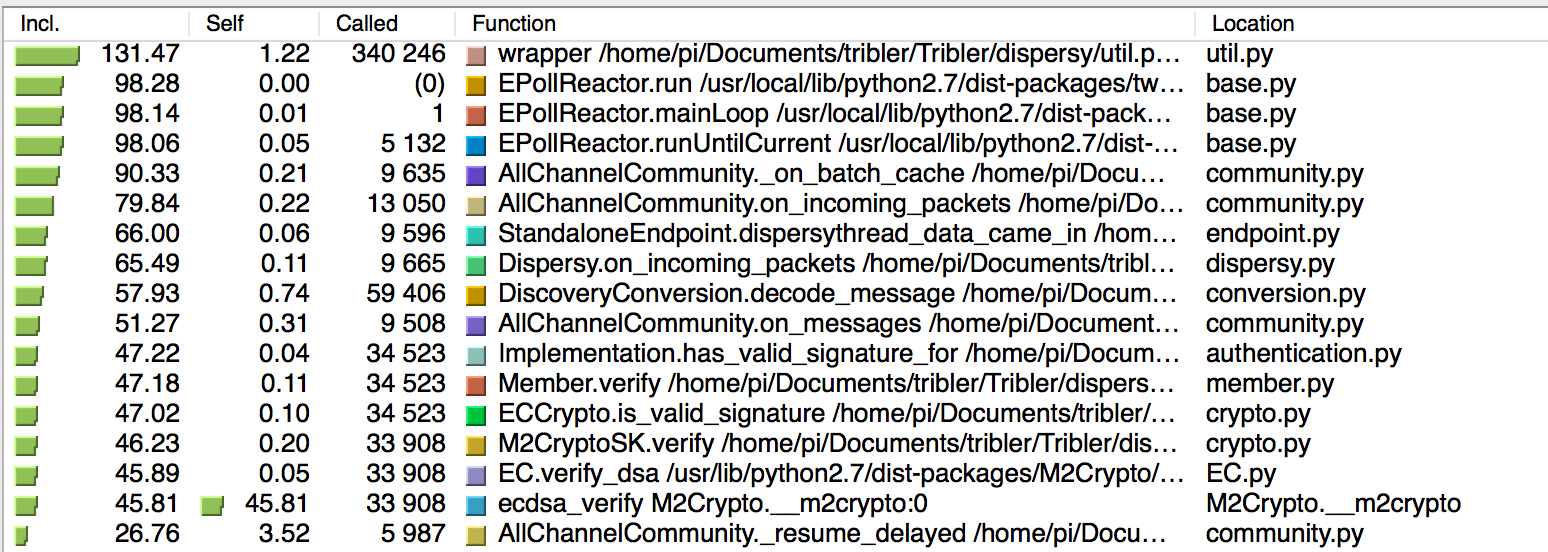
\includegraphics[width=1.0\columnwidth]{images/experiments/yappi_breakdown}
	\caption{The breakdown of method execution times of a 20-minute Tribler run on the Raspberry Pi.}
	\label{fig:yappi_breakdown}
\end{figure}

\noindent In the breakdown presented in Figure \ref{fig:yappi_breakdown}, the \emph{wrapper} method appears to have a huge impact on the performance, being called 340.246 times during our run, however, only 1.22\% of the run time is spent in this method. The method itself is responsible for running specific methods on the reactor thread using a decorator. Many of these decorators can be removed when we remove the old user interface, further explained in Section \ref{sec:threading-model-improvements}. Next, we notice various methods in the \emph{EPollReactor} class. These methods are only calling methods that are scheduled in the event loop of Twisted and the run time of these methods can be neglected.\\\\
Further analysing the breakdown, we notice that Dispersy has a big impact on the performance of Tribler when running on the Raspberry Pi. The \emph{ecdsa\_verify} method (second method from the bottom) is dominating the runtime of Tribler: 45.81\% of the Tribler run time is spent inside the method. This specific method verifies the cryptographic signature of an incoming Dispersy message and is invoked every time a signed message is received. Disabling cryptographic verification of incoming messages should improve the situation, however, this is a trade-off between security and performance: by not verifying incoming messages, fake messages by an adversary can be forged and are accepted without any verification in such a system.\\\\
To verify whether the system load decreases when we disable cryptographic verification of incoming messages, we measure the CPU usage of two different runs. Both runs start with a non-existing Tribler state directory and have a duration of ten minutes. In the first run, we are using the default configuration of Tribler, like in most of the other experiments described in this chapter. In the second run, we disable verification of incoming messages in Dispersy by changing the cryptography option of Dispersy to \emph{NoVerifyCrypto} (by default, this setting is set to \emph{ECCrypto}, specifying that elliptic curves cryptography is used). The CPU utilization over time of the two runs, up to ten minutes are displayed in Figure \ref{fig:raspi_cpu_usage}: on the horizontal axis, we show the time into the experiment and on the vertical axis, we display the CPU utilization in percentage. We emphasize that the Tribler core is limited to run on a single CPU core.\\

\begin{figure}[!h]
	\centering
	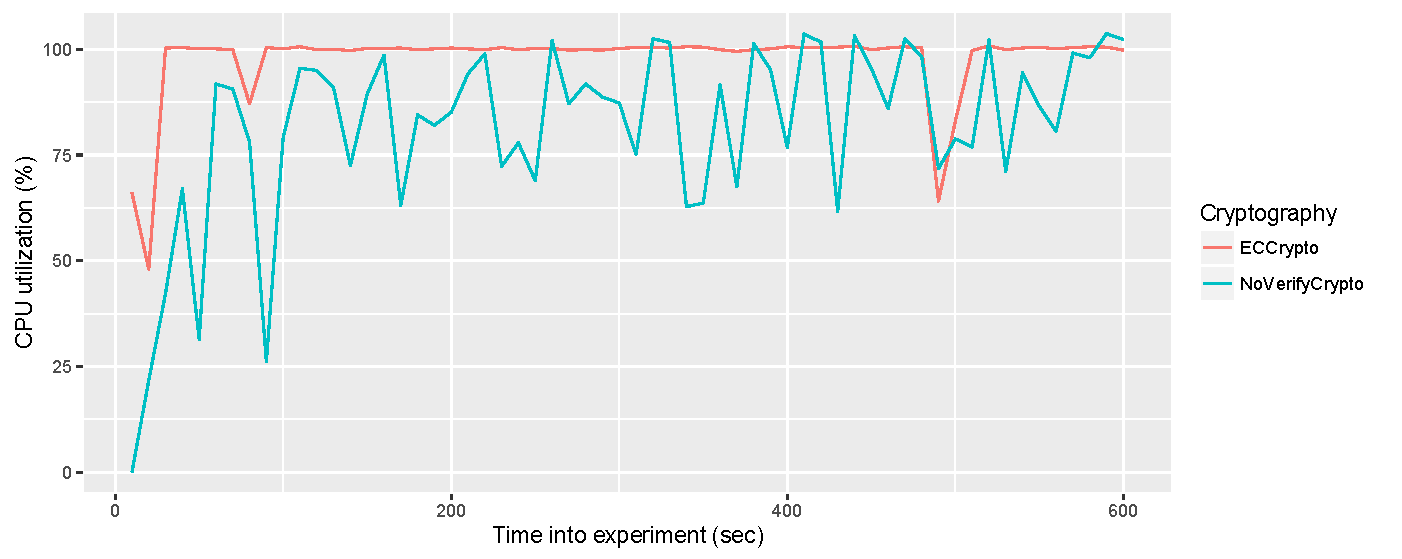
\includegraphics[width=1.0\columnwidth]{images/experiments/raspi_cpu_usage}
	\caption{The CPU utilization of one core on a Raspberry Pi device when running Tribler with and without cryptographic verification of incoming Dispersy messages.}
	\label{fig:raspi_cpu_usage}
\end{figure}

\noindent In Figure \ref{fig:raspi_cpu_usage}, some occurrences can be identified where the CPU utilization appears to be slightly over 100\%. This is explained by the fact that some of the underlying code is designed to run on multiple processors. While the threading model of Tribler is limited to a single core, the Python interpreter might execute code on additional cores to improve performance. In the run where we enable cryptographic verification of incoming messages, the CPU usage is often 100\%, leading to a non-responsive system. When we disable message verification, we observe a somewhat lower CPU usage but overall, this utilization is still relatively high. Unfortunately, disabling incoming message verification is not enough to always guarantee a more usable and responsive system.\\\\
To detect other performance bottlenecks, we sort the report of Figure \ref{fig:yappi_breakdown} on the \emph{self} column to get insights in methods that are taking a long time to complete. This is visible in Figure \ref{fig:yappi_breakdown_self}. An interesting observation is that the Python built-in \emph{all} method takes up a significant amount of time (6.13\% of the runtime). The \emph{all} method takes an iterable object and returns \emph{true} if all objects of this collections resolve to a true value. The \emph{all} method is used in the \emph{\_resume\_delayed} method, indicating that this method might causing performance issues. Since further analysis of this method requires more knowledge of Dispersy, analysis and optimization is considered future work and has been documented in GitHub issue 505\footnote{https://github.com/Tribler/dispersy/issues/505}.\\\\

\begin{figure}[!h]
	\centering
	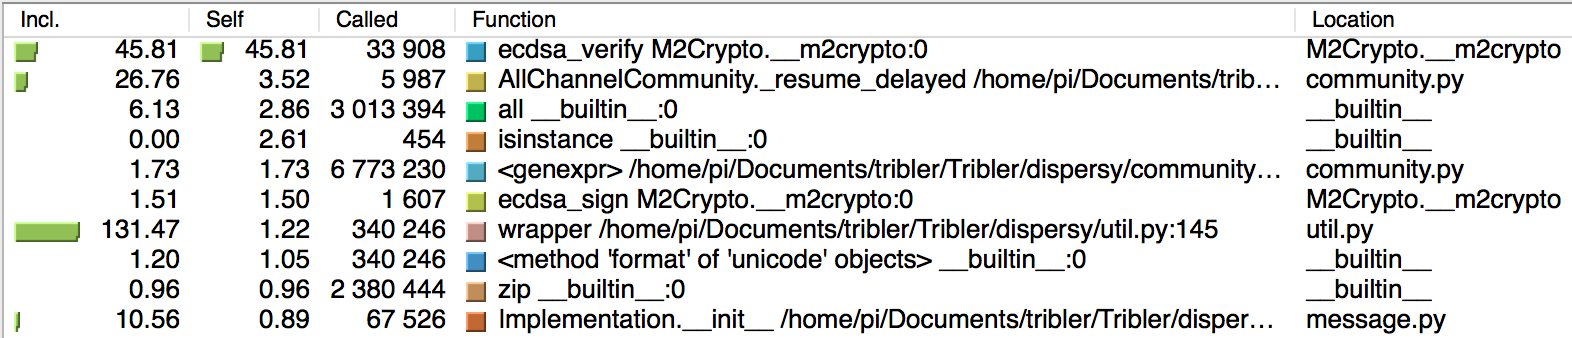
\includegraphics[width=1.0\columnwidth]{images/experiments/yappi_breakdown_self}
	\caption{The breakdown of a 20-minute run of Tribler on the Raspberry Pi, sorted on the \emph{Self} column.}
	\label{fig:yappi_breakdown_self}
\end{figure}

\noindent To summarize, we demonstrated how adequate usage the Yappi profiler can aid with the detection of performance bottlenecks present in Tribler and Dispersy. Integration of the profiler in Tribler makes it convenient for developers to run and analyse Tribler sessions under different circumstances and on a broad range of devices that are able to run Tribler.

\section{Performance of the REST API}
The responsiveness of the REST API is directly influencing the user experience. If response times of API calls are high, users of Tribler have to wait longer before their data is available and visible in the user interface. For this reason, we wish to make the API serve requests as fast as possible. The purpose of this section is to assess the performance of the API with a particular focus on latency of request response times. However, some other statistics will be considered such as average request time, standard deviation of the response times and observed bandwidth. These statistics will help us to get more insights in the performance of the REST API and the responsiveness of Tribler.\\\\
We make use of the Apache JMeter application\footnote{http://jmeter.apache.org} that we configure to perform HTTP requests to Tribler and to gather and process performance statistics. The application allows to simulate a realistic user load, however, in this experiment we will limit the load to one user that performs a request to Tribler with a fixed time interval. The performed (GET) request will be targeted to a specific endpoint in the REST API: \emph{/channels/discovered}. The response of the request consists of a JSON-encoded dictionary of all channels that Tribler has discovered so far. The returned response by this request can be rather large, especially if Tribler has been running for a long time and has discovered many channels (in our experiments, the average response size of the request is around 613KB). We emphasize that the size of the database and thus the response size grows when Tribler is running idle, however, we observed this increase to be at most 1KB, neglectable compared to the response size. During the processing of this request, a database query is performed to fetch all channels that are stored in the persistent SQLite database. This exact request happens when users are clicking the \emph{discover} menu button in the new Qt GUI.\\\\
We perform multiple experiments with different time intervals between requests made and a fixed amount of 500 requests per experiment. First, we conduct an experiment where we perform one request every second and we expect that the system should be able to hand this load and serve these requests in a timely matter. Next, the frequency of requests is increased to respectively 2, 5, 10 and 15 requests per second. Each experiment is started around five seconds after Tribler has started. During the experiment, we are using a pre-filled database with around 100.000 discovered torrents, 1.200 discovered channels and a subscription to 20 channels. A summary of the experimental results are presented in Table \ref{table:performance-api-results} where we display various request statistics.\\

\begin{table}[]
	\centering
	\begin{tabular}{|l|l|l|l|l|l|l|}
		\hline
		\textbf{Requests/sec.} & \textbf{Avg. (ms)} & \textbf{Std. dev. (ms)} & \textbf{Median (ms)} & \textbf{Min. (ms)} & \textbf{Max. (ms)} & \textbf{KB/S} \\ \hline
		\emph{1} & 241 & 476.34 & 76 & 56 & 4246 & 585.58\\ \hline
		\emph{2} & 170 & 327.86 & 68 & 58 & 3394 & 1127.04\\ \hline
		\emph{5} & 123 & 210.23 & 60 & 52 & 2082 & 2538.36\\ \hline
		\emph{10} & 115 & 238.72 & 60 & 50 & 2450 & 4120.70\\ \hline
		\emph{15} & 182 & 497.61 & 68 & 52 & 4937 & 3296.45\\ \hline
	\end{tabular}
	\caption{A summary of the experimental results when measuring the performance of the RESTful API.}
	\label{table:performance-api-results}
\end{table}

\noindent If we focus on the average request time (second column), the most interesting observation is that it appears that requests are served faster if we are performing requests at a faster rate, indicating that Tribler is able to handle the incoming requests well. This is surprising since one would expect this to be the other way around: when the frequency of requests is increased, the average request time is expected to increase since Tribler is under more load, thus increasing request latency. The observed result is most likely explained by caching mechanisms data used by the underlying database engine or Twisted.\\\\
The standard deviation of the request times in Table \ref{table:performance-api-results} (third column) is for all experiments rather high compared to the average request time. We suspect that this can be explained by the fact that Tribler is performing many different operations besides serving API requests. In particular, we think that Twisted is busy with processing other methods that have been scheduled earlier, causing the API requests to be processed later. To verify this, we ran the experiment again where we disable Dispersy, the component responsible for a significant part of the system load (as concluded in Section \ref{sec:profiling_tribler_lowend}). We perform five requests per second and 500 requests in total for this experiment. The observed results are illustrated in Figure \ref{fig:api-performance} where we display the time into the experiment in seconds on the horizontal axis and the request response time in milliseconds on the vertical axis.\\

\begin{figure}[h!]
	\centering
	\begin{subfigure}{.5\textwidth}
		\centering
		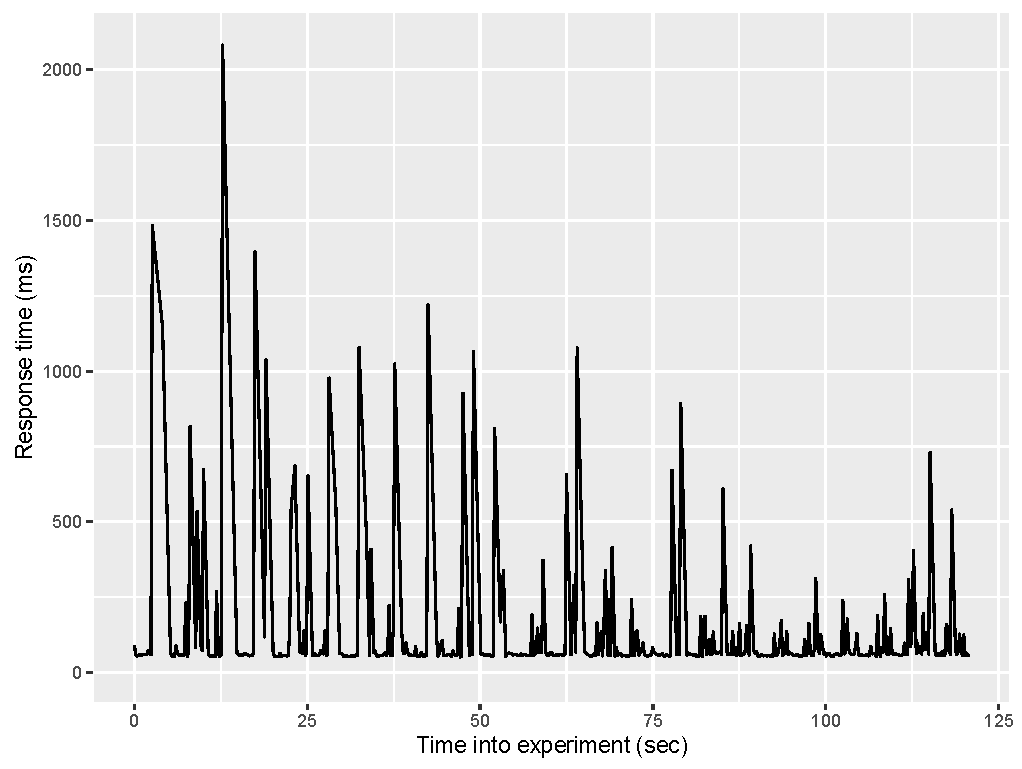
\includegraphics[width=1.0\linewidth]{images/experiments/api_performance_200ms}
		\caption{5 requests/sec, full session}
		\label{fig:api-performance-200ms}
	\end{subfigure}%
	\begin{subfigure}{.5\textwidth}
		\centering
		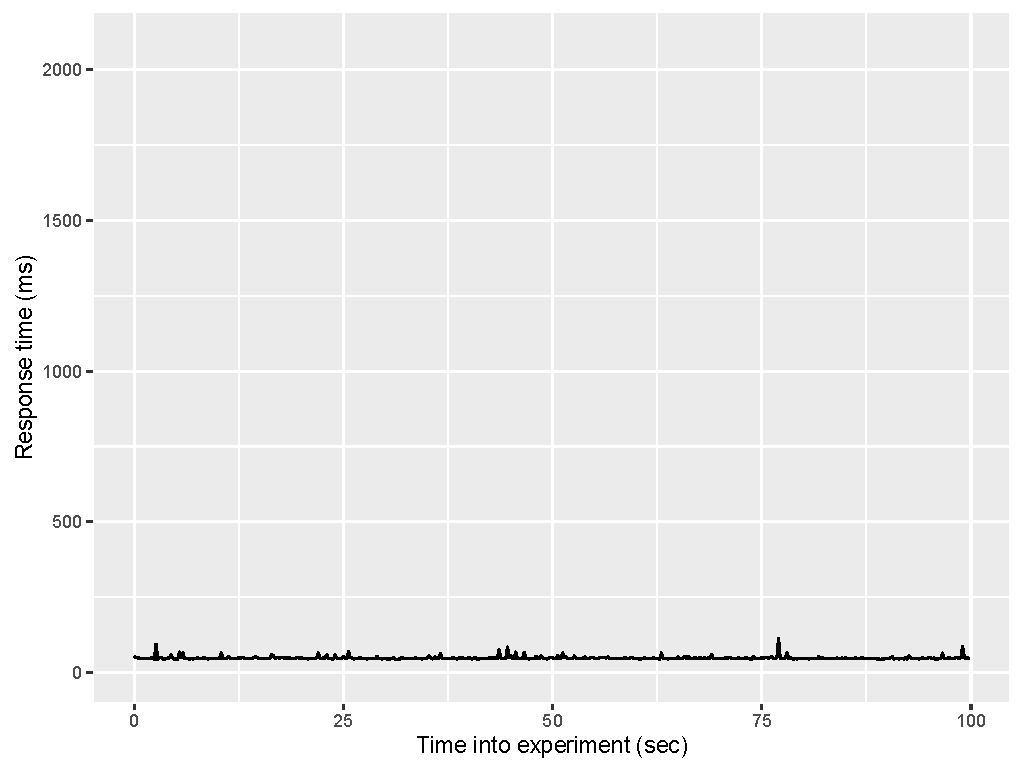
\includegraphics[width=1.0\linewidth]{images/experiments/api_performance_200ms_nodispersy}
		\caption{5 requests/sec, Dispersy disabled}
		\label{fig:api-performance-200ms-nodispersy}
	\end{subfigure}
	\caption{The response times of API requests, in a Tribler session both with Dispersy enabled and disabled.}
	\label{fig:api-performance}
\end{figure}

\noindent In Figure \ref{fig:api-performance-200ms}, the response times of the performed requests with a regular Tribler session is displayed (corresponding to the 5 requests/sec row in Table \ref{table:performance-api-results}) whereas in Figure \ref{fig:api-performance-200ms-nodispersy}, we display the response times of the run with Dispersy disabled. Indeed, the average request time of the requests displayed in Figure \ref{fig:api-performance-200ms-nodispersy} is 48 milliseconds, significantly lower than the average of the response times when Dispersy is enabled, namely 123 milliseconds. The standard deviation in Figure \ref{fig:api-performance-200ms-nodispersy} is 5.73 milliseconds and the standard deviation in Figure \ref{fig:api-performance-200ms} is 210.23 milliseconds. We conclude that the variation in response times is much lower when we disable Dispersy and that Dispersy is producing a huge system load, introducing considerable amounts of latency when performing API requests.\\\\
We identified a key issue here: the latency of methods to be processed in Twisted is high, causing the process operations of incoming requests to be delayed. This is not only a situation that occurs for REST API requests: the same problem is present in Dispersy and the \emph{Tunnel} community where possibly many incoming connections have to be processed and served. A step in the right direction is to make sure that there are no big blocking calls scheduled in Twisted that take a considerable amount of time to complete. When a method with a long execution time is executed, Tribler is unable to process other events during that period, leading to a less responsive system. Ongoing work by another Tribler developer is focussed on making the disk operations in Tribler non-blocking. This should reduce the latency of event processing and improve the responsiveness of the system in general.\\\\
Table \ref{table:performance-api-results} provides us with another interesting observation, namely that it appears that the bandwidth is reducing as the number of requests per second increases. This becomes more obvious if we plot the theoretical maximum bandwidth together with the observed bandwidth during the experiments, see Figure \ref{fig:api-bandwidth-performance}. In this figure, we presented both the obtained bandwidth by running a regular Tribler session and one where Dispersy has been disabled on the vertical axis. The horizontal axis denotes the frequency of the performed requests. We assume that each request contains 613KB (627.712 bytes) of data in the response body. The theoretical maximum obtainable bandwidth is determined as $ b = 613n $ where $ n $ is the number of requests per second and $ b $ is the theoretical maximum bandwidth in KB/s. In practice, we will never reach this theoretical bandwidth since some time is required to initialize the HTTP connection to Tribler which we do not consider in our simple model. Figure \ref{fig:api-bandwidth-performance} clearly shows the impact of a running Dispersy on the bandwidth. Whereas we almost obtain the theoretical bandwidth when we disable Dispersy, the gap between the theoretical maximum and observed bandwidths becomes bigger in the run where we use a full session. When performing fifteen requests every second, the bandwidth even decreases, possibly due to the high system load.\\

\begin{figure}[h!]
	\centering
	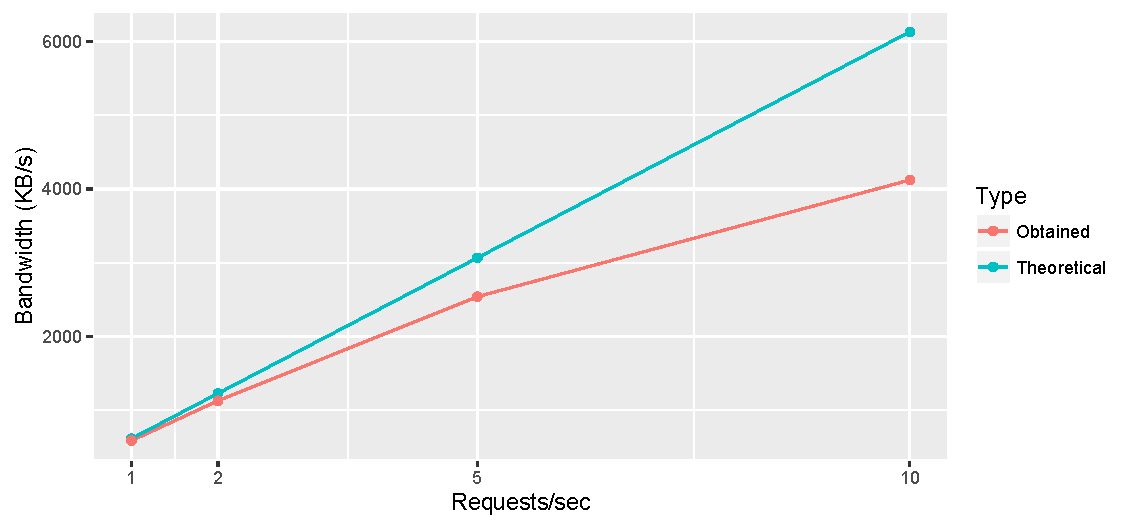
\includegraphics[width=1.0\columnwidth]{images/experiments/api_bandwidth_performance}
	\caption{The theoretical maximum bandwidth compared to the observed bandwidth in the experiments (using a full Tribler session and disabled Dispersy).}
	\label{fig:api-bandwidth-performance}
\end{figure}

\noindent We conclude this experiment with the conclusion that we can use the API response times as a benchmarking tool to measure the responsiveness of the Tribler core. Using the Apache JMeter application, we can easily build a stress test and verify whether performance has increased or decreased after a specific set of modifications. Implementation of such a performance regression framework is considered future work. 

\section{Start-up Experience}
\label{sec:startup-experience}
The first user interaction with Tribler, is the process of booting the software. During this boot process, various operations are performed:
\begin{itemize}
	\item The Tribler state directory where persistent data is stored, is created and initialized with necessary files such as the SQLite database, the Dispersy member key pair and various configuration files.
	\item A connection to the SQLite database is opened and initialized.
	\item Dispersy is initialized and the communities that are enabled in the configuration file are loaded.
	\item Various Tribler components are created and initialized, including the video streaming server, the RESTful API, the remote torrent handler, responsible for fetching torrent information from other peers and a key-value storage for torrent meta info.
\end{itemize}
The start-up process of the Tribler core proceeds sequentially and no parallel operations are implemented to speed up the process. Depending on the enabled components in the configuration file, the start-up time might vary.\\\\
To analyse the start-up time, we perform two experiments where we start Tribler 50 times in a row. In one experiment, the software is started for the first time, with no prior existing state directory. When starting Tribler with no prior existing state directory, a new one is created and the required files are initialized. In the other experiment, a pre-filled database containing just over 100.000 torrents is used. This database has been built by running Tribler idle for several hours, after subscribing to various popular channels to synchronize and discover as much torrents as possible. In both experiments, there are no active downloads. A timer is started when the \emph{start} method of the \emph{Session} object is called and stopped when the notification that Tribler has started, is observed. This allows us to determine the total start-up time of Tribler to a granularity of milliseconds.\\\\
During the span of this thesis, there have been various changes to the start-up procedure of Tribler where code has been modified, removed and added. Since we would like to guarantee that our modifications did not significantly decrease the start-up speed, we make a comparison between the Tribler code in November '15 and July '16. The results are presented in Figure \ref{fig:startup-experiment}, where we present an empirical cumulative distribution function (ECDF) with the boot time in seconds on the horizontal axis and within each plot, the distribution of start-up times from a clean and pre-filled state directory. The ECDF for the distribution of boot times using the November '15 code base is presented in Figure \ref{fig:startup-time-2015} whereas the boot times of the July '16 code base is visible in Figure \ref{fig:startup-time-2016}.\\

\begin{figure}[h!]
	\centering
	\begin{subfigure}[b]{1\textwidth}
		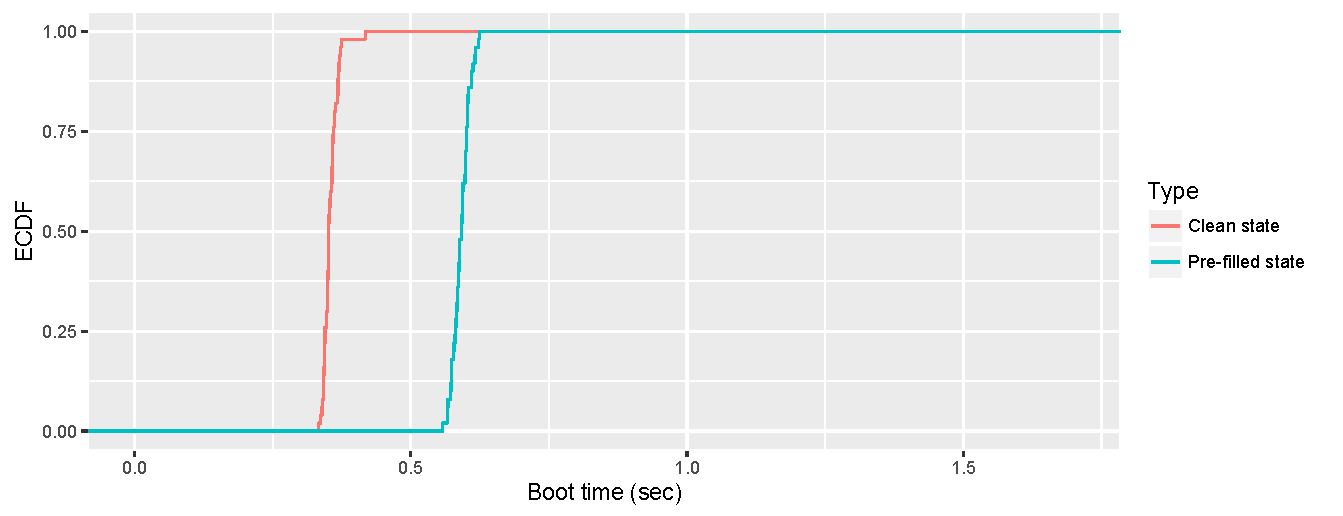
\includegraphics[width=1\linewidth]{images/experiments/startup_time_2015}
		\caption{The boot time of Tribler with the code base of November '15.}
		\label{fig:startup-time-2015} 
	\end{subfigure}
	
	\begin{subfigure}[b]{1\textwidth}
		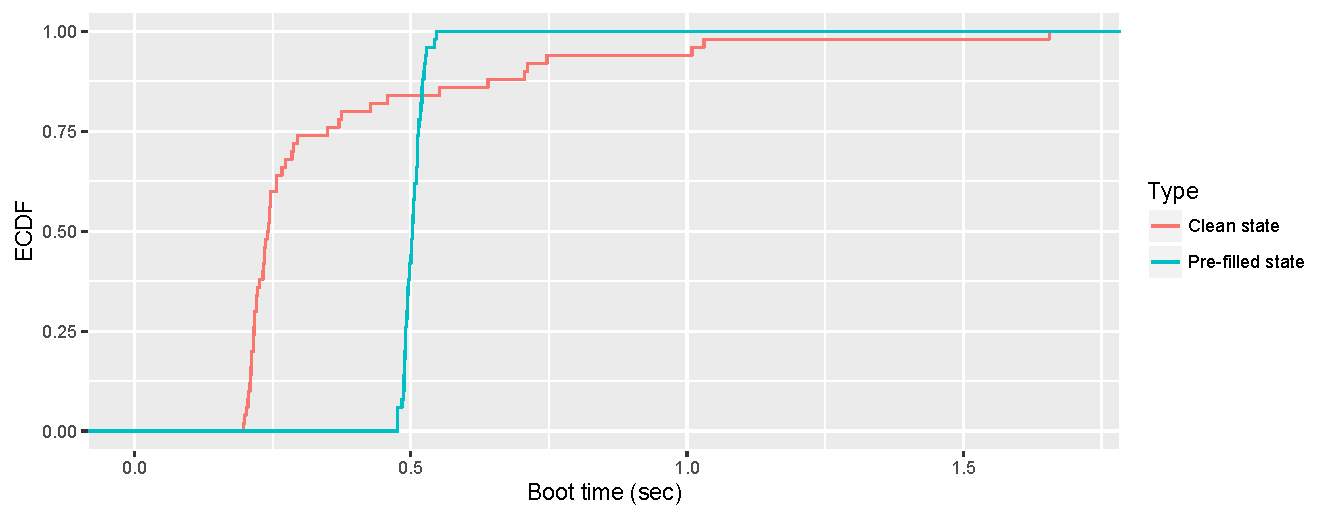
\includegraphics[width=1\linewidth]{images/experiments/startup_time_2016}
		\caption{The boot time of Tribler with the code base of July '16.}
		\label{fig:startup-time-2016}
	\end{subfigure}
	
	\caption{The start-up time of Tribler from a clean and pre-filled state using the code base from November '15 and July '16.}
	\label{fig:startup-experiment}
\end{figure}

\noindent The average start-up times for a clean and filled state using the November 2015 code base are 0.35 and 0.59 seconds respectively. For the July 2016 code, these values are 0.35 and 0.50 seconds. In both plots of Figure \ref{fig:startup-experiment}, It is clear that size of the Tribler database has impact on the boot time of Tribler, however, this impact is relatively minor since the system still starts within a second. We think that this statistic justifies removal of the splash screen that is shown in the old user interface: the duration of the splash screen visibility in the new interface is so short that users would not even be able to read and interpret the content of the splash screen. In contrast to the old user interface, the new GUI starts Tribler and shows a loading screen after the interface has started. However, the difference is that users are able to already perform some basic actions before Tribler has started, such as browsing of discovered content.\\\\
Whereas the boot times of the experiments performed with the November '15 code are very constant, both when using a clean and pre-filled state directory, we notice a larger variation when starting from a clean state in the experiment with the code base from July '16, indicating that there is a component that has a high variation in initialization time during the start-up procedure. Further analysis learns us that this variation can be addressed to Dispersy, possibly caused by the initialization of a community. However, further investigation of the boot time of Dispersy is outside the scope of this thesis work.

\section{Remote Content Search}
\label{sec:remote-content-search-experiment}
We wish to serve relevant information to users as fast as possible. To help users to get content they are interested in, a remote keyword search has been implemented, allowing users to search for torrents and channels inside the Tribler network. Channel results are fetched by a query in the \emph{AllChannel} community whereas torrent results are retrieved by a query in the \emph{Search} community, however, for the experiments in this section, we will focus on remote search for torrents since the amount of channels is rather small compared to the number of torrents available in the network.\\\\
Several experiments to verify the speed of remote torrent search are discussed now. A list of 100 search terms that have a high chance of triggering search results is used and each query is executed when there are at least twenty connected peers in the \emph{Search} community (this condition is checked every second). The time out period of the remote search is 60 seconds, indicating that incoming search results after this period are not regarded (the used search queries are presented in Appendix \ref{appsec:search-remote}). This experiment is focussed on two performance statistics: the time interval until the first remote torrent search result arrives and the turnaround time of the search request, meaning the interval until the last search response arrives. We should note that users performing a remote search might see results earlier since a lookup query in the local database is performed in parallel (the performance of local search is discussed in Section \ref{sec:local-content-search}). The results of our remote search experiment are presented in Figure \ref{fig:remote-search} where we created two ECDF plots with the distributions of time until the first response (Figure \ref{fig:remote-search-first-response}) and time until the last response (Figure \ref{fig:remote-search-last-response}). On the horizontal axis, the measured time interval in seconds is displayed.\\\\
Overall, the remote torrent search as implemented in Tribler is fast and performs reasonable. On average, there are 61 incoming search results for each performed query where the first torrent result takes on average 0.26 seconds to arrive. As we see in Figure \ref{fig:remote-search-first-response}, over 90\% of the first search results are available within a second. During our experiment, we always have the first incoming torrent result within 3.5 seconds. Figure \ref{fig:remote-search-last-response} the turnaround time of the request, indicating the time until the last response within our time out period. On average, it takes 2.1 seconds for all torrent search results to arrive. In Figure \ref{fig:remote-search-last-response}, we notice that in over 90\% of the search queries, we have all results within 10 seconds.\\

\begin{figure}[h!]
	\centering
	\begin{subfigure}{.5\textwidth}
		\centering
		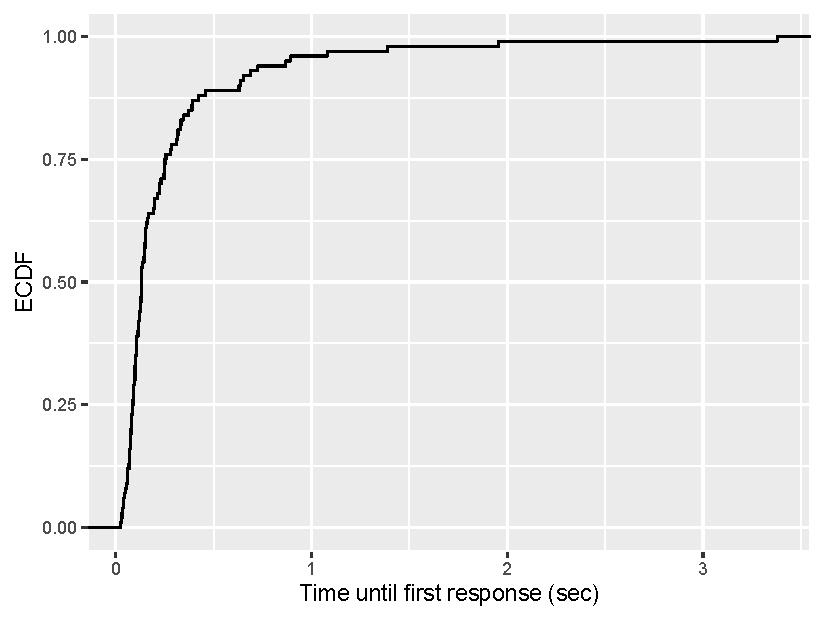
\includegraphics[width=1.0\linewidth]{images/experiments/remote_search_first_response}
		\caption{Times until first response.}
		\label{fig:remote-search-first-response}
	\end{subfigure}%
	\begin{subfigure}{.5\textwidth}
		\centering
		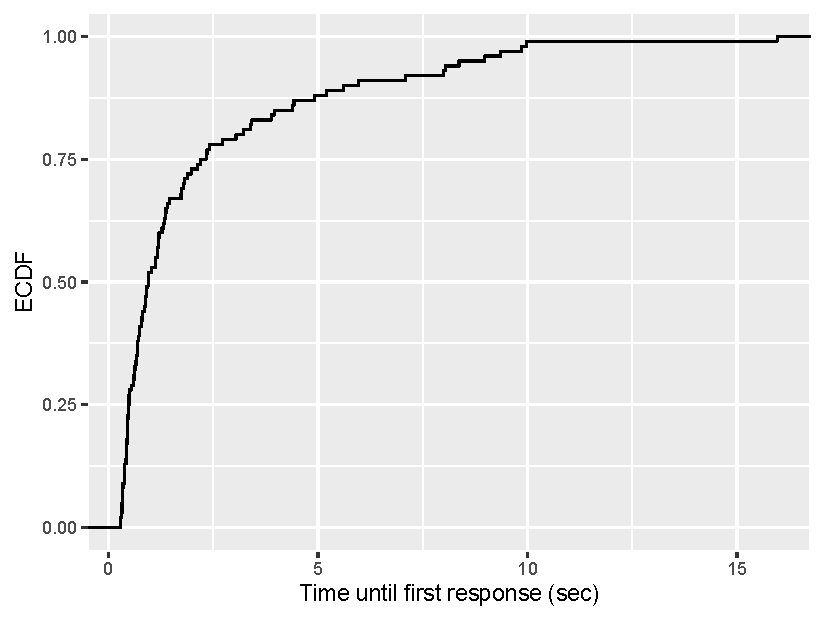
\includegraphics[width=1.0\linewidth]{images/experiments/remote_search_last_response}
		\caption{Times until last response.}
		\label{fig:remote-search-last-response}
	\end{subfigure}
	\caption{The response times of API requests, in a Tribler session both with Dispersy enabled and disabled.}
	\label{fig:remote-search}
\end{figure}

\noindent The same experiment has been performed in 2009 by Nitin et al. where 332 remote search queries have been performed. Their results are presented in an ECDF in Figure \ref{fig:nitin_remote_search} where the time until the first response from any remote peer in the network is measured (the horizontal axis denotes these response times). The graph makes a comparison before and after a significant improvement to the message buffering mechanism, causing messages to be exchanged at a faster rate. The observed average time until first response in 2009 is 0.81 seconds whereas the observed average time in our experiments is 0.26 seconds, more than three times as fast.\\

\begin{figure}[!h]
	\centering
	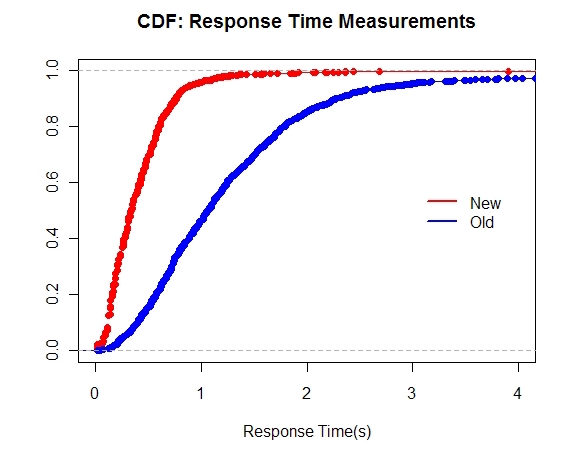
\includegraphics[width=0.7\columnwidth]{images/experiments/nitin_remote_search}
	\caption{The performance of remote content search, performed by Nitin et al. in 2009. The new remote search had an improved input/output mechanism, causing messages to be exchanged faster.}
	\label{fig:nitin_remote_search}
\end{figure}

\noindent We conclude this experiment with the conclusion that the remote search is reliable and fast. We receive an adequate amount of search results and the first remote search results are often available within a second. We might add anonymity to the searches by having other peers (say peer A) perform the search query on behalf of a peer B. If we built an anonymous circuit between peer A and B when peer B wants to perform a remote search, it becomes significantly harder for adversaries to determine which query peer A initiated.

\section{Local Content Search}
\label{sec:local-content-search}
In the previous section, we demonstrated and elaborated the performance of the remote content search mechanism. Now, we will shift the focus to performance measurements of local content search, which is considered more trivial than the remote search counterpart due to the lack of network communication. In particular, our goal is to quantify the performance gain or loss when switching to the new relevance ranking algorithm where we utilized a newer database search engine, as described in Section \ref{sec:relevance-ranking-algorithm}.\\\\
The set-up of this experiment is as follows: a database with just over 100.000 torrents is used. Around ten seconds after starting Tribler, we perform a local torrent search every second and we do this for 1.000 random keywords that are guaranteed to match at least one torrent in our database. We will measure both the time spent by the database lookup and the time it takes for the data to be post-processed after being retrieved from the database. In the code base of November '15, this post-processing step involves determining the associated channels that are containing a specific torrent result. This experiment is performed for the old method that uses the Full Text Search 3 (FTS3) engine and the new procedure that uses the more recent Full Text Search 4 (FTS4) engine. According to the SQLite documentation, FTS3 and FTS4 are nearly identical, however, FTS4 contains an optimization where results are returned faster when performing searches with keywords that are common in the database. The result of the experiments with the old and new local search logic is visible in Figure \ref{fig:local-keyword-search}, presented in two ECDF plots: Figure \ref{fig:local-keyword-search-fts3} gives the distribution of local keyword search times with the old algorithm, using FTS3. Figure \ref{fig:local-keyword-search-fts4} presents the search times of the new local search algorithm, using FTS4. In both plots, the horizontal axis denotes the time of either the database query time (the orange line) or the total time for the processing of results, including the database query time (the blue/green line).\\

\begin{figure}[t]
	\centering
	\begin{subfigure}[b]{1\textwidth}
		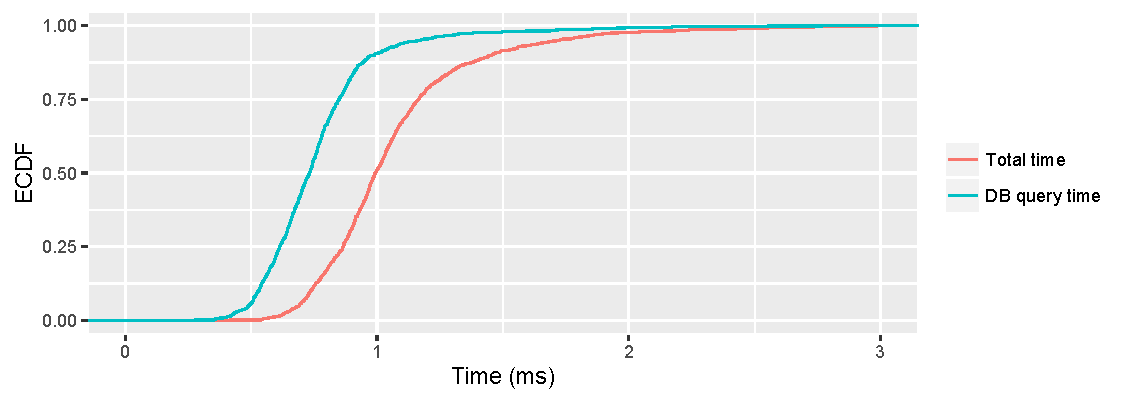
\includegraphics[width=1\linewidth]{images/experiments/local_search_fts3}
		\caption{Local keywords search (FTS3), old algorithm.}
		\label{fig:local-keyword-search-fts3} 
	\end{subfigure}
	
	\begin{subfigure}[b]{1\textwidth}
		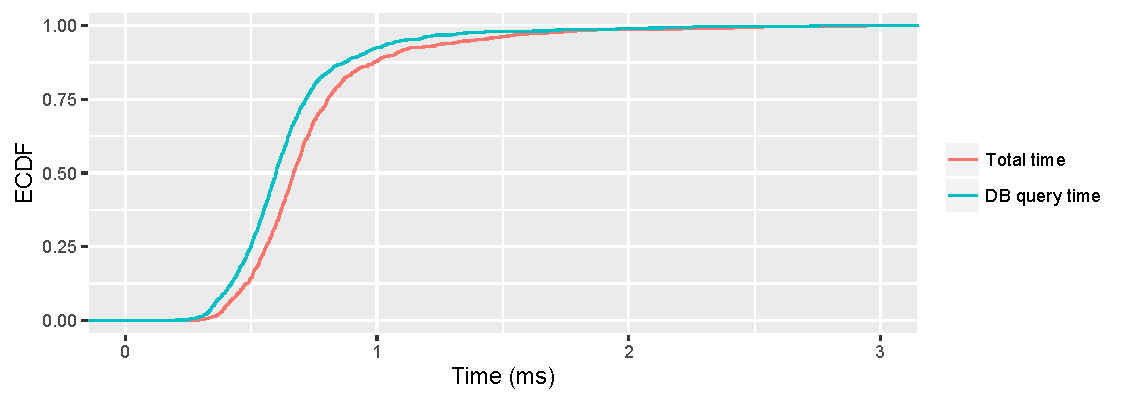
\includegraphics[width=1\linewidth]{images/experiments/local_search_fts4}
		\caption{Local keywords search (FTS4), new algorithm.}
		\label{fig:local-keyword-search-fts4}
	\end{subfigure}
	
	\caption{The distribution of local search durations of the old (FTS3) and new (FTS4) algorithm.}
	\label{fig:local-keyword-search}
\end{figure}

\noindent Local content search is very fast, delivering results in several milliseconds and performance engineering on the local content search engine should not be prioritized. We see that the two lines in the FTS3 and FTS4 plots have moved closer to each other which means that the total time of post-processing of torrent results has decreased. This is in line with our expectations since the new relevance ranking algorithm should be less computationally expensive than the old one. In addition, the new algorithm takes less factors in considering, for instance, the swarm health of the torrent. The increase in performance from FTS3 to FTS4 is visible but not significant.\\\\
In 2009, Nitin et al. performed the same experiment where they used a database filled with 50.000 torrents. Their generated ECDF is displayed in Figure \ref{fig:local-search-nitin}. We notice that the performance of local search in our experiment is dramatically better than the performance obtained during the 2009 experiment, however, we should note that the experiment by Nitin et al. has most probably been performed with older, slower hardware than used in our experiment. Another explanation for the huge differences in local query duration is that Tribler used a custom inverted index implementation when the experiment in 2009 was conducted. An inverted index is a data structure where a mapping is stored from words to their location in the database and is used on a large scale by search engines, including the FTS engine of SQLite. By utilizing this mapping when performing a full text search, we can get results in constant time. However, there is a slight overhead for maintaining and building the inverted index when new entries are added to the database, also impacting the size of the database disk file. The built-in FTS engine of SQLite is optimized to a large extent and clearly offers a higher performance than the custom implementation in 2009.

\begin{figure}[h!]
	\centering
	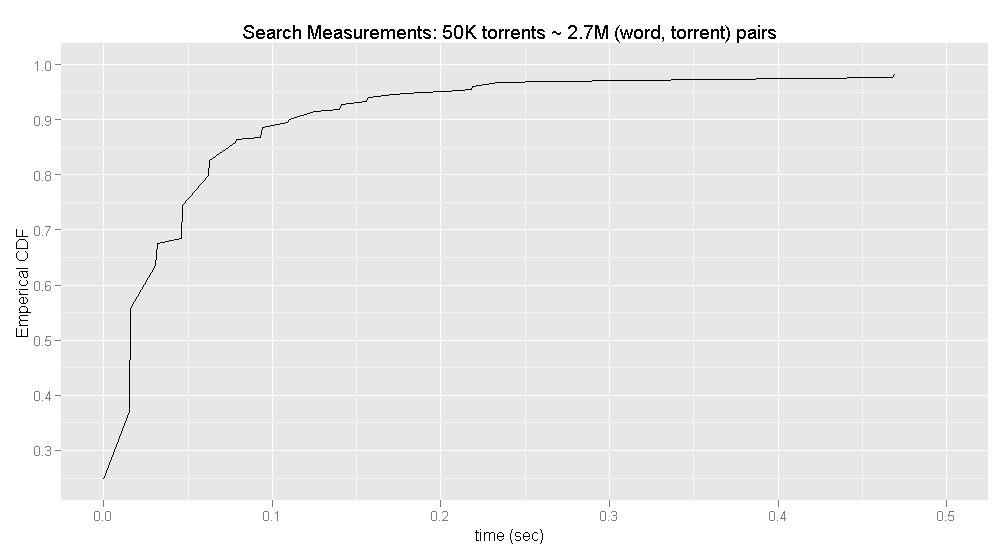
\includegraphics[width=1.0\columnwidth]{images/experiments/nitin_local_search}
	\caption{The performance of a local database query as verified by Nitin et al. in 2009.}
	\label{fig:local-search-nitin}
\end{figure}

\section{Video Streaming}
The embedded video player in Tribler allows users to watch a video that is being downloaded and the inner working is explained in more detail in Section \ref{subsubsec:video-server}. Video playback has been available since Tribler 4.0 and has been implemented using the VLC library. One distinguishable feature is support for seeking so the user can jump to a specified time offset in the video. Video downloads have a special video on demand (VOD) mode which means that the libtorrent piece picking mechanism uses a linear policy mode, downloading pieces in a sequential order. When the user moves to a specified position in the video, the prioritization of the pieces is modified, giving priority to pieces just after the specified seek position. The bytes are streamed to a VLC-compatible client using a HTTP stream. When Tribler starts, a video server is started if enabled in the configuration file. Users do not have to use the built-in player and also have the possibility to use an external video player that support playback of a HTTP video stream.\\\\
To improve user experience, we wish to minimize the delay that users experience when performing a seek operation in the video player. The experiment performed in this section, will quantify this buffering delay. For this purpose, the well-seeded \emph{Big Buck Bunny}\footnote{https://peach.blender.org} movie will be downloaded. The movie file has a size of 885.6 MB and has a duration of 9 minutes and 56 seconds. We will perform various HTTP range requests using the \emph{curl} command line tool\footnote{https://curl.haxx.se}, immediately after starting the download in Tribler (the download is started around ten seconds after Tribler has started). For every run, we will request 10 megabyte of data with different offsets within the file and we will measure the total time it takes for each HTTP request to complete. The results are visible Table \ref{table:video_player_seek_times} where we specified the first requested byte and the time until the request has been fulfilled and the response is received.\\

\begin{table}[]
	\centering
	\begin{tabular}{|l|l|}
		\hline
		\textbf{First byte}               & \textbf{Time until request done (sec)} \\ \hline
		0                        & 11.6                  \\ \hline
		$ 1 * 10^9 $ & 64.4                  \\ \hline
		$ 2 * 10^9 $ & 64.6                  \\ \hline
		$ 3 * 10^9 $ & 65.9                   \\ \hline
		$ 4 * 10^9 $ & 100.6                   \\ \hline
		$ 5 * 10^9 $ & 115.6                   \\ \hline
		$ 6 * 10^9 $ & 115.8                  \\ \hline
		$ 7 * 10^9 $ & 12.2                  \\ \hline
		$ 8 * 10^9 $ & 66.6                   \\ \hline
		$ 9 * 10^9 $ & 52.4                   \\ \hline
	\end{tabular}
	\caption{Performance of the video player when requesting 10MB of data at different byte offsets of a video that is being downloaded.}
	\label{table:video_player_seek_times}
\end{table}

\noindent Theoretically, we would expect around the same request time for each range request, assuming that the availability of each piece is high. When performing a seek operation in the video, the piece picking mechanism adjusts priorities and these prioritized pieces should start to download immediately. The experiments shows various anomalies in this mechanism where it might take up to two minutes for data to be available. Further investigation of this issue learns us that the video player always tries to download the first 10\% of the video file. We found out that this is intended behaviour of the code since the video player needs the information embedded in the file header first. This file header provides information about the file type, file duration and encoding used. There are some video formats where this kind of information is present at the end of the video file.\\\\
We conclude this experiment with the statement that the video player is a very important component in Tribler and requires more attention. Apart from performance gain by integrating the video player in Twisted, we might think about a smarter algorithm to make sure that we download the video file header first. Always downloading the first 10\% of the file might lead to wasted time in case of a large video file if the user jumps immediately to the middle of the video. This situation becomes even worse when we enable the anonymous download overlay, decreasing the download speed and increasing latency before playback of a video starts.

\section{Content Discovery}
\label{sec:content-discovery}
Content discovery is a key feature of Tribler. By running Tribler idle for a while, content is synchronized with other peers using the Dispersy messaging mechanism. When a user starts Tribler for the first time, there is no discovered content yet. We will verify the discovery speed of content after a first fresh start. The experiment is structured as follows: we measure the interval from the completion of the start procedure to the moment in time where the first content (a channel and a torrent) is discovered. The experiment is repeated fifteen times. The results are presented in Figure \ref{fig:content_discovery_speed} where we created an ECDF with a distribution summary of the discovery times of torrents (green line) and channels (orange line). The horizontal axis denotes this channel or torrent discovery time.\\

\begin{figure}[!h]
	\centering
	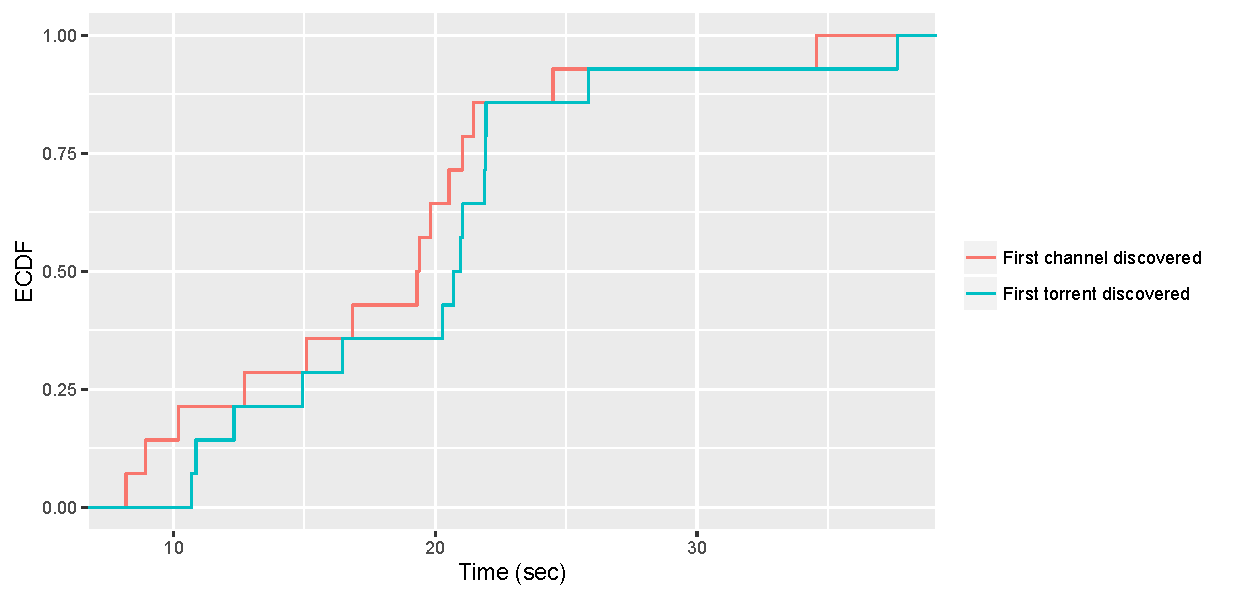
\includegraphics[width=1.0\columnwidth]{images/experiments/content_discovery}
	\caption{The discovery time of the first channel and torrent after starting Tribler for the first time.}
	\label{fig:content_discovery_speed}
\end{figure}

\noindent The delay of discovering the first channel is reasonably: this happens on average 18 seconds after start-up. In all runs, we have our first channel discovered within 35 seconds after Tribler starts. Discovery times of the first torrent is slightly slower and in all runs, the first torrent in a channel is discovered within 40 seconds. Figure \ref{fig:content_discovery_speed} suggests that a torrent discovery always happens after there is at least one discovered channel. This is true: after the channel is discovered, the PreviewChannel community is joined where torrents are exchanged and discovered after a while.\\\\
In the old wxPython user interface, users were presented with a blank screen with no feedback about content that is being discovered in the background. In the new Qt user interface, the user is presented with a screen that informs the user that Tribler is discovering the first content. This screen is only visible the first time Tribler is started and is dismissed when there are five discovered channels after which the page with an overview of discovered channels is presented to the user. We think that it is justifiable for users to wait until some channels have been discovered before they can perform actions: the time they have to wait is relatively short (around 30 seconds) and the waiting period could be combined with a small tutorial about Tribler (this feature is not implemented in the first iteration of the new Qt interface).

\section{Channel Subscription}
When Tribler runs idle, not all available content in the network is discovered. The majority of torrents is discovered when users subscribe to a channel (in the old user interface, this is equivalent to marking a channel as favourite). When Tribler discovers a new channel, users are able to browse through a preview of this channel. Internally, Tribler connects to the PreviewChannel community associated with that channel, a community derived from the channel community. In this preview community, the amount of torrents that are collected is limited. The channel community is joined the moment the user subscribes to a channel, after which all available content is synchronized. Removing the preview mechanism might significantly increases the resource usage of the Tribler session since the amount of incoming messages to be decoded and verified will increment.\\\\
The experiment as described in this section, will focus on the discovery speed of additional content after the user subscribes to a specific channel and on the resource allocation when we are running Tribler without enabling the preview mechanism of channels. For the first experiment where we determine the discovery speed of additional content inside a channel, the twenty most popular channels (having the most subscribers) are determined. To get these channels, we have used a Tribler state directory with many discovered channels but void of any channel subscriptions. Exactly ten seconds after Tribler started, we subscribe to one of these popular channels and we measure the time interval between subscription to the channel and the first additional torrent discovered. Tribler is restarted between every run and the state directory is cleaned so we guarantee a clean state of the system. The observed results are visible in an ECDF displayed in Figure \ref{fig:channel-subscription} with the time until torrent discovery on the horizontal axis.

\begin{figure}[!h]
	\centering
	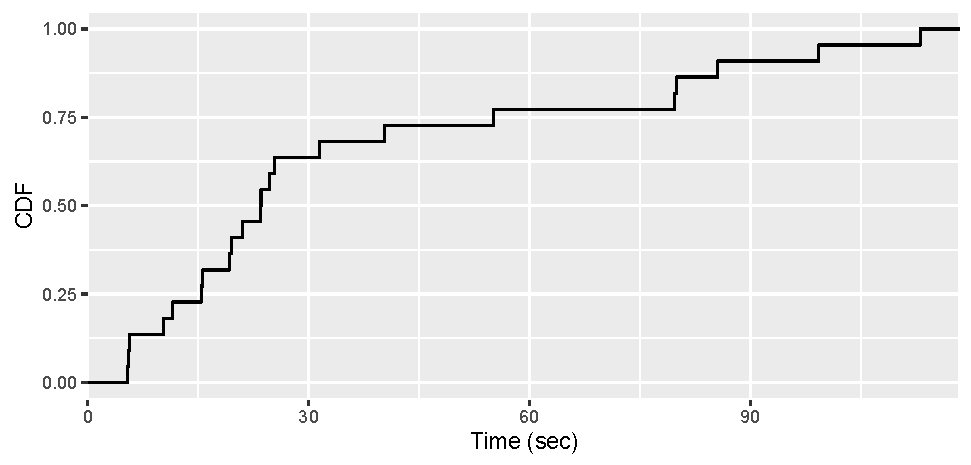
\includegraphics[width=1.0\columnwidth]{images/experiments/channel_subscription}
	\caption{An ECDF of discovery times of the first additional torrent after subscribing to a popular channel.}
	\label{fig:channel-subscription}
\end{figure}

\noindent The average discovery time of additional torrents after subscription to a channel is 36.8 seconds which is quite long, compared to the discovery speed of the first channel and torrent after start up as described in Section \ref{sec:content-discovery}. The discovery times have a high variation as can be seen in Figure \ref{fig:channel-subscription}. This can be explained by the fact that immediately after subscribing to a channel, Tribler will connect to the channel community and it takes some time for new peers to be discovered.\\\\
To verify the impact of automatically subscribing to each channel and synchronizing all content when it is discovered, we perform a CPU utilization measurement. In two idle runs of a Tribler session, both lasting for ten minutes, we measure the CPU utilization every ten seconds using output provided by the \emph{top} tool. In the first run, a regular Tribler session is used where previews of discovered channels are enabled. In the second run, we bypass the preview of a discovered channel and immediately join the channel community, synchronizing all available content. Both types of runs start with an empty state directory. The results of this experiment are visible in Figure \ref{fig:channel-subscription-cpu} where we display the time into the experiment in seconds on the horizontal axis, up to ten minutes and the CPU utilization in percentage on the vertical axis. We display both the utilization with channel previews enabled and disabled.

\begin{figure}[!h]
	\centering
	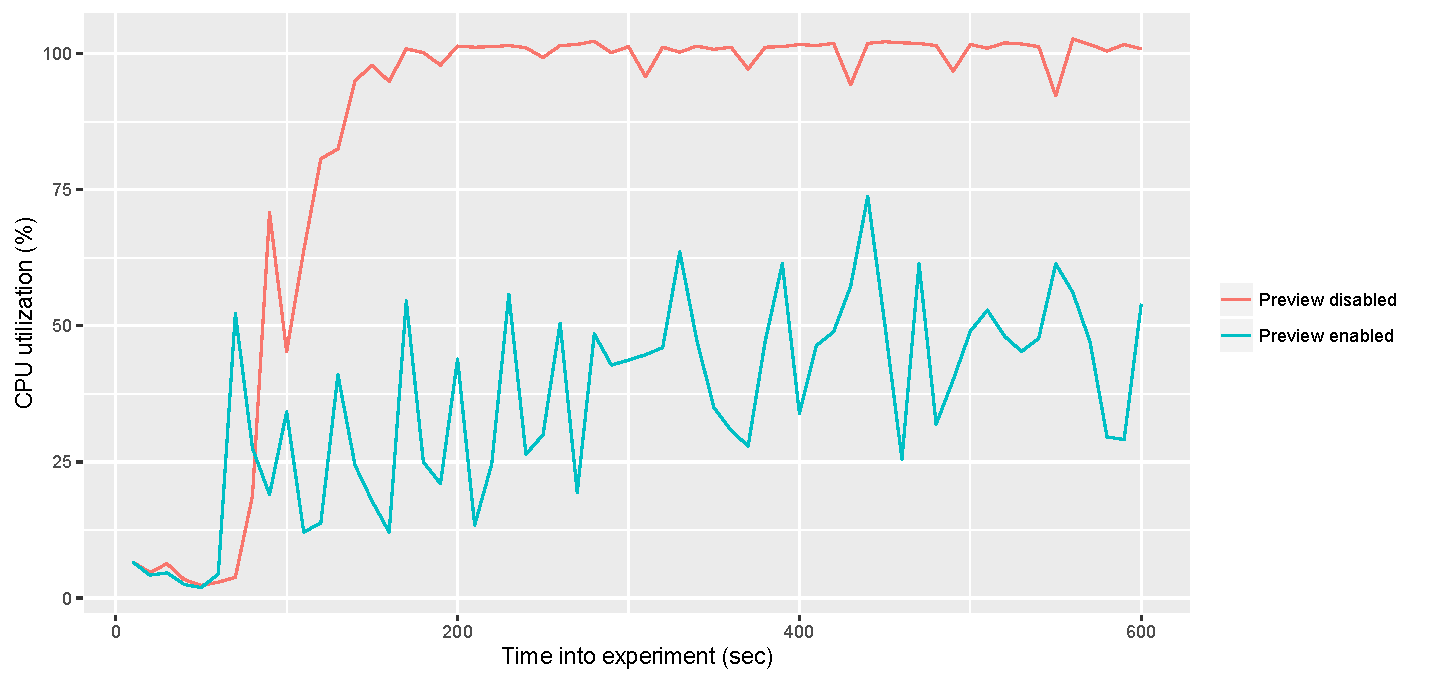
\includegraphics[width=1.0\columnwidth]{images/experiments/subscribe_cpu_experiment}
	\caption{The CPU utilization of one core during a period of ten minutes with channel preview enabled and disabled.}
	\label{fig:channel-subscription-cpu}
\end{figure}

\noindent Whereas the CPU usage of the normal run is around 45\% on average, the CPU is quickly rising to 100\% utilization when we enable the auto-join mechanism of channels. This shows that it is infeasible to enable this auto-join feature if we still wish to guarantee a responsive system. One might limit the rate at which discovered torrents are fetched, however, this requires a feedback mechanism where we should notify other peers in the community to limit the amount of messages sent to the peer that is discovering content. Implementation of such as feature is outside the scope of this thesis work and is considered future work.

\section{Torrent Availability and Lookup Performance}
While specific information about torrents such as the name and file names are distributed within the Dispersy communities, this does not hold for the meta info about the torrent itself, which includes additional data such as available trackers and piece information. This meta info might be important for users since trackers provides information about the health of a torrent swarm. The experiments as performed in this section, will investigate the torrent availability and lookup performance of meta info of torrents, both by downloading them from remote peers in the Tribler network and when querying the \emph{Distributed Hash Table (DHT)}.

\subsection{Trivial File Transfer Protocol Handler}
When users are performing a remote torrent search, the first three incoming results are pre-fetched in the old user interface which means that the meta info of these torrents are fetched automatically. An incoming search result from the Dispersy network might contain information about remote peers (candidates) that have meta info of this torrent available. If candidates for a specific remote torrent result are present, an attempt to fetch the torrent meta info from this candidate is scheduled. This request is performed using the TFTP mechanism\cite{sollins1992tftp}. TFTP is also used to transfer meta data about torrent files such as thumbnails between peers, however, the exchange of torrent meta data is currently disabled in Tribler. The implementation of TFTP is located in the Tribler core package.\\\\
There has been no published studies yet about the performance of our TFTP implementation so we have no reference material. The experiment performed in this section will focus on the performance of TFTP when fetching meta info from remote peers. We start from a clean state directory and exactly one minute after starting Tribler, we perform a remote torrent search. For each incoming remote search result, we perform a TFTP request. We perform ten remote torrent search operations in total, with interval of 60 seconds between them (the used search queries can be found in Appendix \ref{appsec:search-queries-tftp}). For every incoming result, we schedule a remote torrent lookup with a priority of 0. A TFTP request is performed every five seconds. After eleven minutes, we stop Tribler and gather the statistics of the TFTP sessions. The observed results are presented in Table \ref{table:tftp-performance}, where we display the total amount of scheduled requests, requests still in the queue, the number of failed requests and the amount of succeeded requests.\\

\begin{table}[h!]
	\centering
	\begin{tabular}{|l|l|}
		\hline
		\emph{Total requests scheduled} & 1008 \\ \hline
		\emph{Requests in queue} & 761 (75.5\%)\\ \hline
		\emph{Requests failed} & 106 (10.5\%)\\ \hline
		\emph{Requests succeeded} & 141 (14.0\%)\\ \hline
	\end{tabular}
	\caption{A breakdown of the final state of the performed requests during the TFTP performance measurement.}
	\label{table:tftp-performance}
\end{table}

\noindent We notice that the queue keeps growing: when our experiment is finished, 75.5\% of the initiated requests is still in the queue. We must emphasize that we are scheduling requests at a rather fast rate. The second observation is the high failure rate when compared to the amount of succeeded requests (42.9\% if we do not consider the requests in the queue). We identified two underlying reasons for the failed requests: first, some of the requests timed out, possibly due to the fact that several remote peers are not connectible. A solution for this kind of failure would be a robust NAT puncturing method. The second reason is that the remote peer might not have the requested file in the local persistent storage. While this situation might seem unusual, it can happen if the remote peer has the requested torrent information in the SQLite database but not in their meta info store, a separate persistent database used to store binary torrent files. We can solve this by not returning the peer as candidate if the torrent is not available in the meta info store. This solution might reduce the total bandwidth used by the TFTP component.\\\\
Next, we will focus on the turnaround time of successful TFTP requests, presented in the ECDF in Figure \ref{fig:tftp-performance-success}. This ECDF only considers requests that have succeeded and the horizontal axis denotes the total time in seconds it took before the TFTP request has been finished. We notice the weird distribution of the turnaround times: we would expect that the total request times to fetch meta info using TFTP is somewhat constant, however, we see outgoing requests that take over 400 seconds to complete. This trend will probably continue if we did not stop the experiment after eleven minutes. The most reasonable explanation for this is that requests are added to the request queue at a faster rate than the processing speed of these requests. This also explains the values denoted in Table \ref{table:tftp-performance} where 75.5\% of the request are still in the queue after the experiment ends. Better support for parallel requests should help, however, this is considered further work.

\begin{figure}[!h]
	\centering
	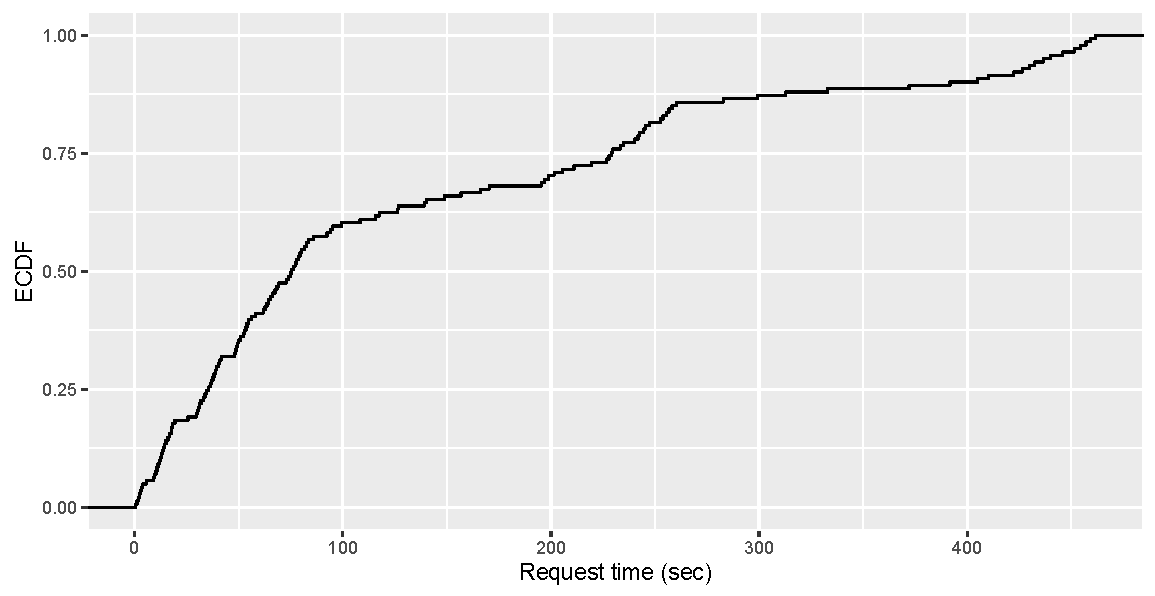
\includegraphics[width=1.0\columnwidth]{images/experiments/tftp_performance}
	\caption{An ECDF of the performance of the torrent meta info download mechanism using TFTP in Tribler.}
	\label{fig:tftp-performance-success}
\end{figure}

\subsection{Distributed Hash Table}
\label{subsec:dht-experiment}
Another additional source of torrent meta info is the DHT. In the DHT, we can lookup meta info of a torrent. In this section, we will perform an experiment to get insights in the availability of torrent files and the performance of lookup operations in the DHT. Like in the TFTP experiment described in the previous section, we wish this meta info to be available as soon as possible to the user.\\\\
For this experiment, a popular channel with over 5.000 torrents is used and a subset of 1.000 random torrent infohashes in this channel is determined. We start Tribler from a clean state and every 40 seconds, a DHT query is performed with one of the 1.000 random infohashes. The time out period used in Tribler is 30 seconds, after which a failure callback is invoked and an error is displayed in the user interface to notify the user about the failed request. The results of this experiments are visible in the ECDF depicted in Figure \ref{fig:metainfo_fetch} where the horizontal axis denotes the request time in seconds before the DHT lookup is completed.\\

\begin{figure}[!h]
	\centering
	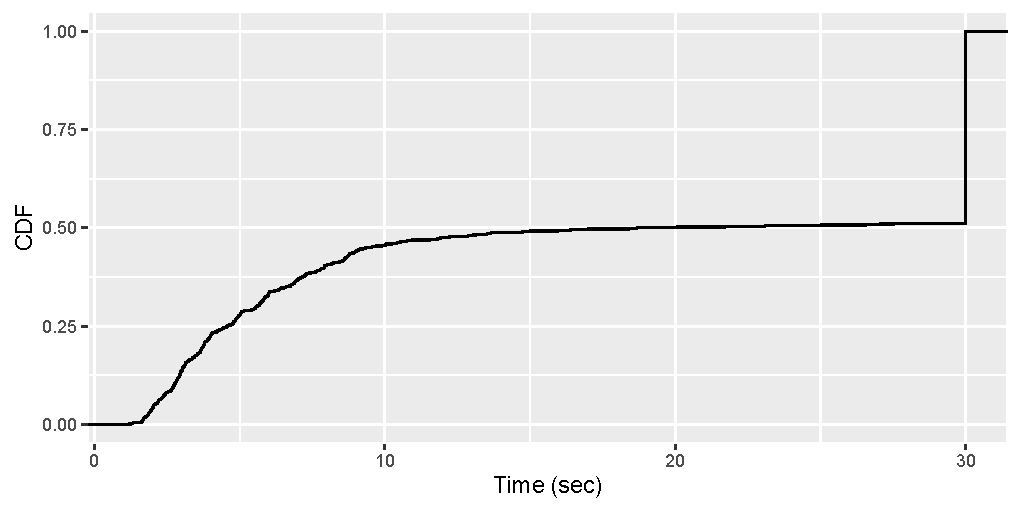
\includegraphics[width=1.0\columnwidth]{images/experiments/metainfo_fetch}
	\caption{An ECDF of the lookup times of torrents in the DHT.}
	\label{fig:metainfo_fetch}
\end{figure}

\noindent We immediately notice that the failure rate of DHT lookups is high: 48.9\% of the lookup operations are timing out and never succeed. This issue might be addressed to dead torrents (when no peers in the DHT have this torrent information available) or private torrents (torrents which information is not exposed in the DHT). The amount of failures might even be higher if we repeated the experiment with torrents in a less popular channel since the content in these channels are likely to be less seeded. As explained in the previous section, the DHT is not the only source for torrents in Tribler and we might also fetch torrents from other peers using TFTP. Unfortunately, the approach of fetching meta info about torrents from other peers is only useful when performing a remote search for torrents whereas the DHT can always be queried. Caching and exchanging torrent candidates is not successful since the availability of candidates cannot be guaranteed.\\\\
The average lookup time of torrents that are successfully fetched from the DHT is 5.81 seconds which is reasonably fast. Additionally, a little over 90\% of the successfully fetched torrents are retrieved within 10 seconds.\\\\
To improve performance of meta info lookups, dead torrents should be handled correctly. One possible solution might be an implementation of a periodical check for each incoming torrent. By limiting the number of outstanding DHT requests, this approach does not require much additional resources. To further improve performance, the result of DHT lookups might be disseminated to remote peers in the network. Torrents that are not successfully fetched from the DHT, could be hidden automatically in the user interface. The downside of this approach is that it might not give a realistic view of the availability of a torrent since their might be Dispersy peers which have information about this torrent available.